\documentclass[prx,twocolumn]{revtex4-2}

\usepackage{amsmath}
\usepackage{amssymb}
\usepackage{graphicx}
\usepackage{braket}

\usepackage{tikz}
\usetikzlibrary{quantikz}

\usepackage{caption}
\usepackage{subcaption}

\usepackage{float}

\numberwithin{equation}{section}
\numberwithin{figure}{section}
\numberwithin{table}{section}

\renewcommand{\theequation}{\arabic{section}.\arabic{equation}}
\renewcommand{\thefigure}{\arabic{section}.\arabic{figure}}
\renewcommand{\thetable}{\arabic{section}.\arabic{table}}

\DeclareMathOperator{\CNOT}{CNOT}
\DeclareMathOperator{\CZ}{CZ}
\DeclareMathOperator{\tr}{tr}

\begin{document}
%Title of paper
\title{Implementing Quantum Teleportation on a Real Quantum Computer using Qiskit \\ Physics 707 Term Paper}
\author{Swagat Kumar}
\affiliation{University of Wisconsin-Madison}
\date{\today}

\begin{abstract}
The quantum teleportation protocol allows two parties to transfer a qubit state from one qubit to another
by sharing only classical information and a pair of qubits in an entangled state. In this paper, I will show 
how to emulate the teleportation protocol to run on IBM's free to use quantum computers using their open source
software development kit -- Qiskit. Lastly, I will use quantum state tomography to measure the fidelity of the 
teleportation protocol on the \textit{ibmq\_5\_yorktown} system which is one of the IBM Quantum Canary processors.
\end{abstract}

\maketitle

\section{The Quantum Teleportation Protocol}
Alice and Bob each have one of two qubits that are in the Bell state 
$\ket{\Psi}_{AB} = \frac{1}{\sqrt2}(\ket0_A\ket0_B + \ket1_A\ket1_B)$.
Alice also has another qubit in the state $\ket\psi = \alpha\ket0+\beta\ket1$, the teleportation protocol allows
her to transfer or \textit{teleport} her state $\ket\psi$ to Bob's qubit by making a measurement on both of 
her qubits. \cite{nielsen-chuang,Qiskit-Textbook} Doing so does not violate the no-cloning theorem as the state 
of Alice's qubit is collapses after measurement. The protocol is described using the quantum circuit in 
Figure \ref{fig:teleportation-circuit}.

\begin{figure}[h]
    \centering
    \begin{quantikz}[scale=1.5]
        \lstick{$\ket\psi_C$} \qw & \ctrl{1} %\slice{$\ket{\psi_1}$} 
        & \gate{H} %\slice{$\ket{\psi_2}$} 
        & \meter{$c_0$} & \cw & \cw & \cwbend{2} \\
        \lstick[wires=2]{$\ket\Psi_{AB}$} \qw & \targ{} & \qw & \meter{$c_1$} & \cw & \cwbend{1}\\
                                          \qw & \qw     & \qw & \qw           & \qw & \gate{X^{c_1}} & \gate{Z^{c_0}} & \qw \rstick{$\ket\psi_B$}
    \end{quantikz}
    \caption{The circuit describing the quantum teleportation protocol.}
    \label{fig:teleportation-circuit}
\end{figure}

The initial state of the system is 
\begin{equation}
    \begin{aligned}
    \ket{\psi_0}    &= \ket\psi_C \otimes \ket\Psi_{AB} \\
                    %&= (\alpha\ket0_C + \beta\ket1_C) \otimes \frac{\ket0_A\ket0_B + \ket1_A\ket1_B}{\sqrt2} \\
                    &= \frac{\alpha}{\sqrt2} (\ket0_C\ket0_A\ket0_B + \ket0_C\ket1_A\ket1_B) \\
                    &+ \frac{\beta}{\sqrt2} (\ket1_C\ket0_A\ket0_B + \ket1_C\ket1_A\ket1_B)
    \end{aligned}
\end{equation}
After Alice applies a CNOT the state evolves to:
\begin{equation}
    \begin{aligned}
    \ket{\psi_1}    &= \CNOT_{C,A} \ket{\psi_0} \\
                    &= \frac{\alpha}{\sqrt2} (\ket0_C\ket0_A\ket0_B + \ket0_C\ket1_A\ket1_B) \\ 
                    &+ \frac{\beta}{\sqrt2} (\ket1_C\ket1_A\ket0_B + \ket1_C\ket0_A\ket1_B)
    \end{aligned} 
\end{equation}
And then after the Hadamard gate:
\begin{equation}
    \begin{aligned}
    \ket{\psi_2}    &= H_C \ket{\psi_1} \\
                    % &= \frac{\alpha}{2} (
                    %     (\ket0_C + \ket1_C)\ket0_A\ket0_B + 
                    %     (\ket0_C + \ket1_C)\ket1_A\ket1_B) \\
                    % &+ \frac{\beta}{2} (
                    %     (\ket0_C - \ket1_C)\ket1_A\ket0_B + 
                    %     (\ket0_C - \ket1_C)\ket0_A\ket1_B) \\ \\
                    &= \frac{1}{2}
                        \begin{bmatrix}
                        \quad \ket0_C\ket0_A (\alpha\ket0_B+\beta\ket1_B) \\
                        +\ket0_C\ket1_A (\alpha\ket1_B+\beta\ket0_B) \\
                        +\ket1_C\ket0_A (\alpha\ket0_B-\beta\ket1_B) \\
                        +\ket1_C\ket1_A (\alpha\ket1_B-\beta\ket0_B)     
                        \end{bmatrix} \\
                    &= \frac{1}{2} 
                    \begin{bmatrix}
                        \ket0_C\ket0_A \otimes \ket\psi_B \\
                        +\ket0_C\ket1_A \otimes X\ket\psi_B \\
                        +\ket1_C\ket0_A \otimes Z\ket\psi_B \\ 
                        \quad +\ket1_C\ket1_A \otimes XZ\ket\psi_B 
                    \end{bmatrix}
    \end{aligned}
    \label{eq:psi-2}
\end{equation}
After applying these gates, Alice measures qubit $C$ to get a bit $c_0$ and measures qubit $A$ to get a bit 
$c_1$. These measurements project Alice's qubits into one of the four 2-qubit standard basis states and
simultaneously project's Bob's qubit into a state that is closely related to $\ket\psi$, as per Equation 
\ref{eq:psi-2}. Alice sends the measured bits to Bob via a classical communication channel, which tells Bob 
the corrective gates he needs to apply to transform his qubit into the state $\ket\psi$, given in Table 
\ref{tab:corrective-gates}.

\begin{table}[h]
    \centering
    \begin{tabular}{|c|c||c|}
        \hline 
        $c_0$ & $c_1$ & Corrective Gate \\ \hline \hline 
        0 & 0 & $I$ \\ \hline
        0 & 1 & $X$ \\ \hline
        1 & 0 & $Z$ \\ \hline
        1 & 1 & $ZX$ \\ \hline
    \end{tabular}
    \caption{The corrective gates Bob needs to apply based on the bits he receives from Alice.}
    \label{tab:corrective-gates}
\end{table}

\section{Teleportation on IBM's Quantum Computers}
As of right now, IBM's quantum computers don't support classically controlled gates \cite{Qiskit-Textbook} 
like the corrective gates that Bob needs to apply in the teleportation protocol. As a result, we can't
directly implement the protocol on an IBM quantum computer because teleportation requires the classical 
communication channel. However, it is possible to emulate the teleportation protocol via a quantum circuit 
that does not have any classically controlled gates and is equivalent to the one in 
Figure \ref{fig:teleportation-circuit}.
\subsection{Principle of Deferred Measurement}
The principle of deferred measurement states that measurements made in the middle of a quantum circuit can 
always be shifted to the end of the circuit, where any classically controlled gates dependent on those 
measurements are replaced by conditional quantum gates. \cite{nielsen-chuang}

\begin{figure}[H]
    \centering
    \begin{subfigure}[b]{0.4\columnwidth}
        \resizebox*{\textwidth}{!}{
        \begin{quantikz}
            \qw & \meter{} & \cwbend{1} \\
            \qw & \qw      & \gate{U} & \qw
        \end{quantikz}
        }
    \end{subfigure}
    \begin{subfigure}[b]{0.4\columnwidth}
        \resizebox*{\textwidth}{!}{
        \begin{quantikz}
            \qw & \ctrl{1} & \meter{} & \cw \\
            \qw & \gate{U} & \qw      & \qw
        \end{quantikz}
        }
    \end{subfigure}
    \caption{The two circuits are equivalent as per the deferred measurement principle.}
    \label{fig:deferred-measurement}
\end{figure}

Making use of this principle, we can construct the following quantum circuit that will emulate the 
teleportation protocol.

\begin{figure}[H]
    \centering
    \begin{quantikz}
        \lstick{$\ket\psi_C$}             & \ctrl{1} & \gate{H} \slice{$\ket{\psi_2}$} & \qw      & \ctrl{2} \slice{$\ket{\psi_3}$} & \meter{$c_0$} & \cw \\
        \lstick[wires=2]{$\ket\Psi_{AB}$} & \targ{}  & \qw      & \ctrl{1} & \qw      & \meter{$c_1$} & \cw \\
                                          & \qw      & \qw      & \targ{1} & \gate{Z} & \qw           & \qw 
    \end{quantikz}
    \caption{The quantum circuit that will emulate the teleportation protocol on the IBM machine.}
    \label{fig:emulated-circuit}
\end{figure}

From Equation \ref{eq:psi-2}, it's clear that after applying the CNOT and controlled-$Z$ gates, the 
system will be in the state
\begin{equation}
    \resizebox{0.9\hsize}{!}{
    $\begin{aligned}
    \ket{\psi_3}    &= \CZ_{C,B} \CNOT_{A,B} \ket{\psi_2} \\
                    &= \frac{\ket0_A\ket0_B + \ket0_A\ket1_B + \ket1_A\ket0_B + \ket1_A\ket1_B}{2}\otimes\ket\psi_C
    \end{aligned}$
    }
\end{equation}

And so, regardless of the measurement outcome, qubit $B$ will be in the state $\ket\psi$. 

\section{Measuring the Teleportation Fidelity of IBM's Quantum Computer}
Unlike the implementation on simulators, we won't have access to the state vector of Bob's qubit at the end 
of running the protocol when we run it on an actual quantum computer. We can however, take multiple 
measurements on different runs of the protocol attempting to reconstruct Bob's state.
\subsection{Quantum State Tomography}
``Quantum state tomography is the attempt to discover the quantum-mechanical state of a physical system, or
more precisely, of a finite set of systems prepared by the same process.'' \cite{tomography}

The state of a single qubit can be characterized with a $2\times 2$ density matrix
\begin{equation}
    \rho = \frac{1}{2} (I + \bar{x} X + \bar{y} Y + \bar{z} Z)
\end{equation}
where $X, Y$ and $Z$ are the Pauli matrices and 
\begin{equation}
    \begin{aligned}
        \bar{x} &= \tr(X\rho), \\
        \bar{y} &= \tr(Y\rho), \\
        \bar{z} &= \tr(Z\rho),
    \end{aligned}
\end{equation}
are the average values of the observables $X,Y$ and $Z$ respectively \cite{nielsen-chuang}.
$\vec{r} = (\bar{x},\bar{y},\bar{z})$ is called the Bloch vector of $\rho$. 
$\|\vec{r}\| \leq 1$, with equality holding only for pure states \cite{nielsen-chuang}.

We can find an approximation of the Bloch vector for a state $\rho$ by instantiating $3N$ qubits in the state 
$\rho$, measuring the observables $X, Y$ and $Z$ on $N$ instances each, and then taking the mean value of the 
observations. We can use this procedure to tomographically reconstruct the state of Bob's qubit after the 
teleportation protocol is finished.

IBM's hardware only allows the measurement of $Z$, with measurement outcome 0 denoting the eigenvalue $+1$ 
and 1 denoting the eigenvalue $-1$. The following circuits can be used to measure $X$ and $Y$.
\begin{figure}[h]
    \centering
    \begin{subfigure}[b]{0.4\columnwidth}
        \resizebox*{0.7\textwidth}{!}{
            \begin{quantikz}
                \qw & \gate{H} & \meter{} & \cw 
            \end{quantikz}
        }
        \caption{$X$ measurement}
    \end{subfigure}
    \begin{subfigure}[b]{0.4\columnwidth}
        \resizebox*{\textwidth}{!}{
            \begin{quantikz}
                \qw & \gate{S^\dagger} & \gate{H} & \meter{} & \cw 
            \end{quantikz}
        }
        \caption{$Y$ measurement}
    \end{subfigure}
    \caption{Circuits to measure $X$ and $Y$ for a qubit.}
\end{figure}

\begin{equation}
    S^\dagger = \begin{pmatrix}
        1 & 0 \\ 
        0 & -i
    \end{pmatrix}
\end{equation}

For a particular observable, say $X$, we can approximate the corresponding Bloch vector coordinate as 
\begin{equation}
    \bar{x} = \frac{N_0 - N_1}{N},
\end{equation}
where $N_0$ is the number of times we note the measurement outcome 0 and $N_1$ the number of times we note 
the measurement outcome 1.

\subsection{Fidelity Calculation}
Through the process described in the previous subsection, we obtain a density matrix $\rho$ that approximates 
the state of Bob's qubit at the end of the teleportation protocol. If Alice had initialized her qubit to the 
pure state $\ket\psi$ at the beginning of the protocol, the fidelity between the $\ket\psi$ and $\rho$ is 
\cite{nielsen-chuang}
\begin{equation}
    F(\ket\psi, \rho) = \sqrt{\bra\psi \rho \ket\psi}.
    \label{eq:fidelity}
\end{equation}

\subsection{Results}
I decided to run my circuits on the \textit{ibmq\_5\_yorktown} system which has 5 qubits as shown in 
\ref{fig:qubit-layout}. The basis gates of the system are $I, R_z, \sqrt{X}, X, \CNOT$ and Reset to $\ket0$.
\begin{figure}
    \centering
    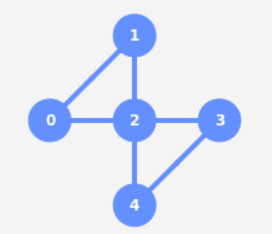
\includegraphics{images/qubit-architecture.png}
    \caption{Layout of the 5 qubits of the \textit{ibmq\_5\_yorktown} system. The vertices represent the qubits 
    and an edge between the qubits means that a physical CNOT gate can be implemented on the connected qubits.}
    \label{fig:qubit-layout}
\end{figure}

This system offers two optimization levels for transpiling a circuit to run on the system -- level 0 where 
the gates of the source circuit are directly converted to the system's basis gates and level 1 where the 
level 0 circuit is optimized for a lower gate count. The transpiled circuit for the emulated teleportation
protocol, shown in Figure \ref{fig:transpiled-circuits}, is independent of the optimization level, but the
circuit to initialize an arbitrary state and the $Y$ measurement circuits have a reduced gate count when 
transpiled at optimization level 1.

\begin{figure*}
    \centering
    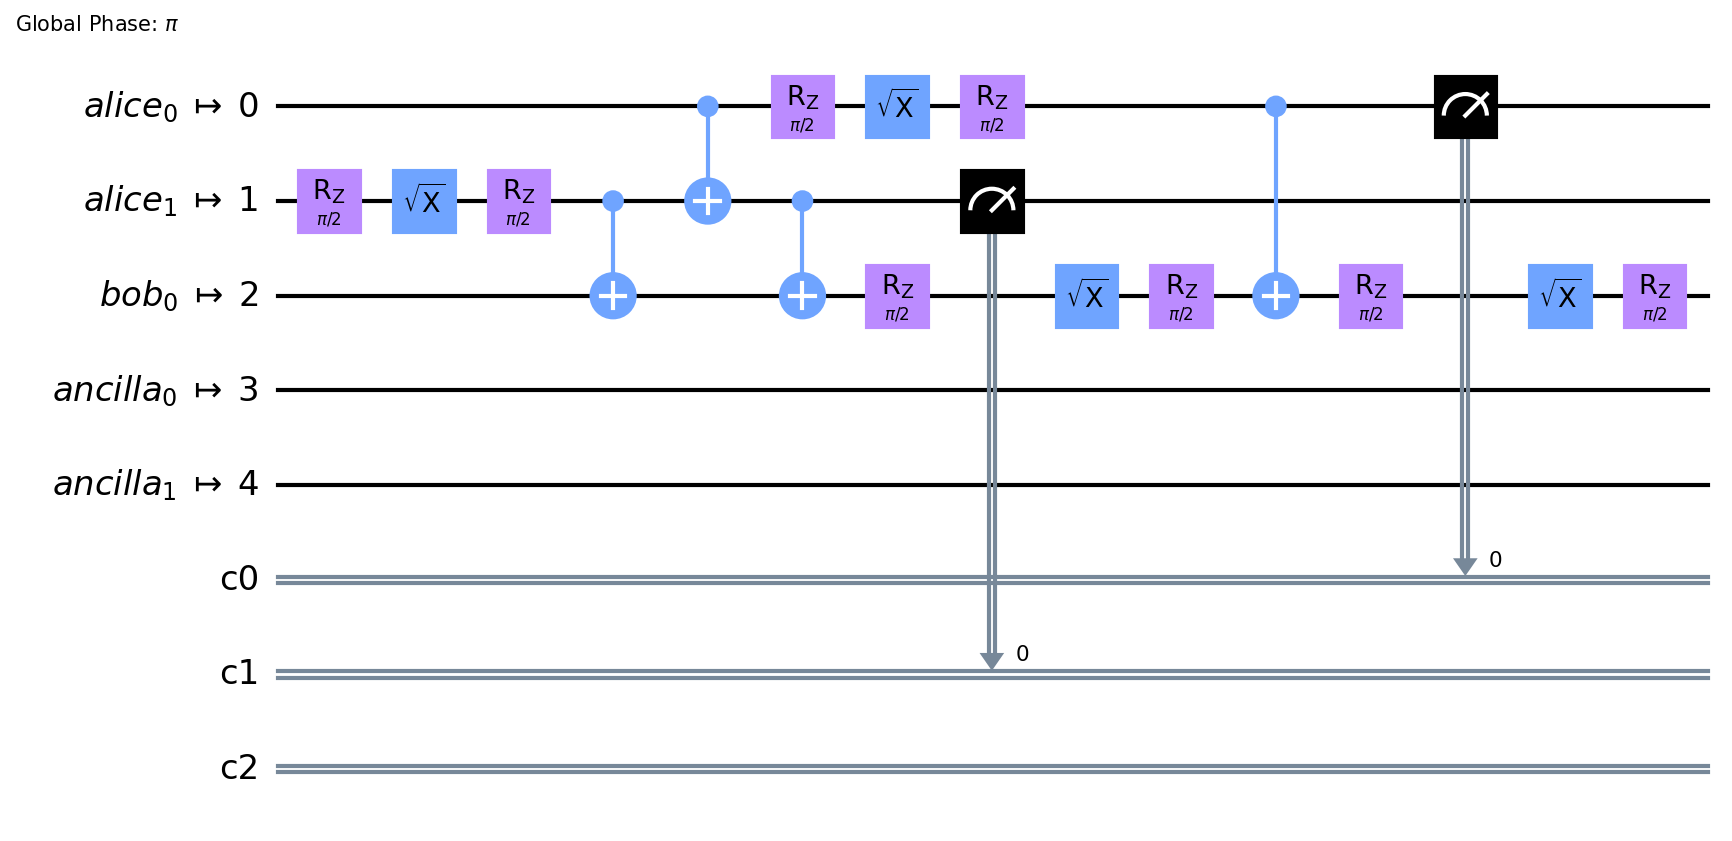
\includegraphics[width=\textwidth]{images/teleport_circ_opt_0.png}
    \caption{The transpiled circuit for the emulated quantum teleportation protocol.}
    \label{fig:transpiled-circuits}
\end{figure*}

For the experiment, I generated 50 random single-qubit states to run the teleportation protocol on. For each 
state, I made $N = 1000$ $X, Y$ and $Z$ measurements each to tomographically reconstruct Bob's state at the 
end of the protocol and calculate the fidelity as per Equation \ref{eq:fidelity}.
\begin{figure}[H]
    \centering
    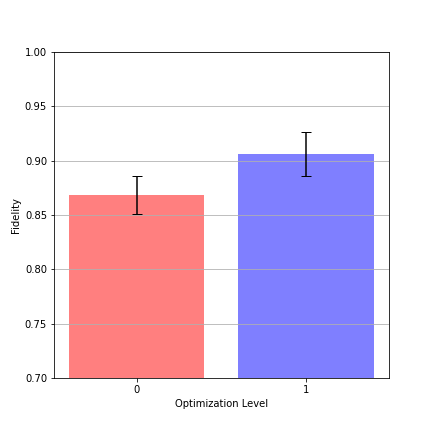
\includegraphics[width=\columnwidth]{images/fidelity-vs-optimization-bar.png}
    \caption{Average fidelities of the teleportation protocol at the two optimization levels.}
\end{figure}

At optimization level 0, the mean fidelity of the protocol was 86.84\% and at optimization level 1, the 
mean fidelity of the protocol was 90.59\%.

\nocite{ibm-quantum}

\begin{acknowledgments}
    I acknowledge the use of IBM Quantum services for this work. The views expressed are those of the author, 
    and do not reflect the official policy or position of IBM or the IBM Quantum team.
\end{acknowledgments}

% Create the reference section using BibTeX:
\bibliography{kumar-swagat-707-term-paper}

\end{document}
%
% ****** End of file apstemplate.tex ******